\everymath{\displaystyle}

%%%%%%%%%%%%%%%%%%%%%%%%%%%%%%%%%%%%%%%%
%           main body
%%%%%%%%%%%%%%%%%%%%%%%%%%%%%%%%%%%%%%%%

%-----------------------------------
%	TITLE PAGE
%-----------------------------------

\title[第三章\\
可测函数]{\texorpdfstring{\LARGE \bfseries 第三章\quad 可测函数}{第三章 可测函数}}
\author[\S 3.2\\
可测函数列的收敛性]
{\Large \bfseries \S 3.2 可测函数列的收敛性}
\date{}

%------------------------------------------------

\begin{document}

%------------------------------------------------

\begin{frame}

\titlepage

\end{frame}

%------------------------------------------------

\section{引言}

%------------------------------------------------

\begin{frame}{引言: 收敛有多少种意义?}

\textbf{回顾}: \S 3.1 中可测函数列最自然的收敛是\alert{逐点收敛} (零测集外成立即为 a.e.\ 收敛); 数学分析里还有\alert{一致收敛} --- 它保证极限函数连续、极限运算可交换等.

\pause

\begin{question}
a.e.\ 收敛比一致收敛弱得多, 二者相差多远? 能否找到一个\alert{更弱}、却仍带\alert{完备性}的收敛概念?
\end{question}

\pause

\textbf{本节路线图}:
\begin{itemize}
\item 工具: 集列的上极限集 / 下极限集 (\S 1.1 已介绍), 把``不收敛''翻译成``无穷多次坏'';
\item a.e.\ 收敛的\alert{测度刻画} (引理) $\Longrightarrow$ \alert{Egorov 定理}: $mE<\infty$ 时, a.e.\ 收敛 = 挖掉任意小测度集后的一致收敛;
\item 更弱的新概念: \alert{依测度收敛} (打字机函数列); F.~Riesz 定理、极限的唯一性、\alert{完备性}、运算性质.
\end{itemize}

\textbf{约定}: 以下 $f, f_k\ (k \in \mathbb{N})$ 均为可测集 $E$ 上 a.e.\ 有限的可测函数, 特别声明除外.

\end{frame}

%------------------------------------------------

\section[上下极限]{集列的上、下极限集}

%------------------------------------------------

\begin{frame}{回顾: 集列的上极限集与下极限集 (\S 1.1)}

\begin{Def}[上、下极限集]
对集列 $\{A_n\}$:
\[
\varlimsup_{n\to\infty} A_n = \bigcap_{k=1}^{\infty}\ \bigcup_{n=k}^{\infty} A_n,
\qquad
\varliminf_{n\to\infty} A_n = \bigcup_{k=1}^{\infty}\ \bigcap_{n=k}^{\infty} A_n.
\]
\end{Def}

\pause

\begin{itemize}
\item $x \in \varlimsup_{n} A_n \iff x$ 属于\alert{无穷多个} $A_n$;
\item $x \in \varliminf_{n} A_n \iff$ \alert{从某项起}恒有 $x \in A_n$ (至多有限个 $A_n$ 不含 $x$);
\item $\varliminf_{n} A_n \subset \varlimsup_{n} A_n$; 二者相等时称集列收敛, 公共集为 $\lim\limits_{n} A_n$.
\end{itemize}

\pause

\begin{attnblock}
本节的关键用法 --- 把``不收敛''翻译成坏集合列的上极限: 固定 $\varepsilon > 0$, 若 $x$ 属于无穷多个 $E(|f_k - f| \geqslant \varepsilon)$, 则 $f_k(x) \not\to f(x)$, 即
\[
\bigcap_{n=1}^{\infty}\ \bigcup_{k \geqslant n} E(|f_k - f| \geqslant \varepsilon)
\ \subset\
\{x \in E:\ f_k(x) \not\to f(x)\}.
\]
\end{attnblock}

\end{frame}

%------------------------------------------------

\section{Egorov 定理}

%------------------------------------------------
% 引理: a.e. 收敛的测度刻画 (Egorov 定理的引擎)

%------------------------------------------------

\begin{frame}{引理: a.e.\ 收敛的测度刻画}

\begin{lem}[a.e.\ 收敛的测度刻画]
设 $f, f_k$ 是可测集 $E$ 上 a.e.\ 有限的可测函数, $mE < \infty$, 且 $f_k \xrightarrow{\text{a.e.}} f$. 则 $\forall\, \varepsilon > 0$, 记
\[
E_k(\varepsilon) := E(|f_k - f| \geqslant \varepsilon),
\]
有
\[
\lim_{n\to\infty}\ m\Big(\bigcup_{k \geqslant n} E_k(\varepsilon)\Big) = 0 .
\]
\end{lem}

\pause

\begin{itemize}
\item $E_k(\varepsilon)$ 可测: $f_k - f$ 可测 (\S 3.1 四则运算), 再取 $|\cdot|$ 与水平集;
\item $\bigcup_{k \geqslant n} E_k(\varepsilon)$ = ``第 $n$ 项之后\alert{至少坏一次}''的点集; 让 $n \to \infty$, 得``\alert{无穷多次坏}''的点集 --- 集列上极限语言;
\item 结论: 对每个固定的 $\varepsilon$, ``无穷多次坏''的点集为零测集 --- a.e.\ 收敛的\alert{定量化}.
\end{itemize}

\end{frame}

%------------------------------------------------

\begin{frame}{引理的证明 (一): 化为渐缩集列}

\startproof[bg=yellow, fg=red](证明)
记 $G_n := \bigcup_{k \geqslant n} E_k(\varepsilon)$, 则
\[
G_1 \supset G_2 \supset \cdots \supset G_n \supset \cdots
\]
是\alert{渐缩}可测集列, 且
\[
mG_n \leqslant mE < \infty \qquad (\text{\alert{此处用到 } mE < \infty}).
\]

\pause

由测度对渐缩集列的\alert{上连续性} (\S 2.3):
\[
\lim_{n\to\infty} mG_n = m\Big(\bigcap_{n=1}^{\infty} G_n\Big).
\]

于是只需证 $\bigcap_{n} G_n$ 是零测集. (下页)

\qed

\begin{attnblock}
渐缩连续性中 $mG_1 < \infty$ 不可少: $G_n = (n, +\infty)$ 时 $mG_n \equiv +\infty$, 而 $\bigcap_n G_n = \emptyset$ (\S 2.3 反例).
\end{attnblock}

\end{frame}

%------------------------------------------------

\begin{frame}{引理的证明 (二): 交集零测}

\startproof[bg=yellow, fg=red](证明 (续))
任取 $x \in \bigcap_{n=1}^{\infty} G_n$, 则 $x$ 属于\alert{无穷多个} $E_k(\varepsilon)$:
\[
\forall\, N,\ \exists\, k \geqslant N:\quad |f_k(x) - f(x)| \geqslant \varepsilon,
\]
故 $f_k(x) \not\to f(x)$.

\pause

所以
\[
\bigcap_{n=1}^{\infty} G_n
\ \subset\
\{x \in E:\ f_k(x) \not\to f(x)\}
\ \subset\ Z, \qquad mZ = 0,
\]
是零测集.

\pause

代回上页:
\[
\lim_{n\to\infty} m\Big(\bigcup_{k \geqslant n} E_k(\varepsilon)\Big)
= m\Big(\bigcap_{n=1}^{\infty} G_n\Big) = 0 .
\]
\qed

\end{frame}

%------------------------------------------------

\begin{frame}{Egorov 定理}

\begin{thm}[Egorov]
设 $f, f_k$ 是可测集 $E$ 上 a.e.\ 有限的可测函数, $mE < \infty$, 且 $f_k \xrightarrow{\text{a.e.}} f$. 则 $\forall\, \delta > 0$, 存在 $E$ 的可测子集 $E_\delta$, 使得
\begin{itemize}
\item[(1)] $m(E \setminus E_\delta) < \delta$;
\item[(2)] $\{f_k\}$ 在 $E_\delta$ 上\alert{一致}收敛于 $f$.
\end{itemize}
\end{thm}

\pause

\begin{Def}[近一致收敛]
满足 (1)(2) 的 $\{f_k\}$ 称为在 $E$ 上\alert{近一致收敛}于 $f$ (almost uniform convergence).
\end{Def}

\pause

\textbf{解读}: a.e.\ 收敛与一致收敛之间的鸿沟, 在 $mE < \infty$ 时只是一``\alert{小测度集合}'': 任意抛弃测度小于 $\delta$ 的集合后, 收敛就是一致的.

\end{frame}

%------------------------------------------------

\begin{frame}{Egorov 定理的证明 (一): 构造 $E_\delta$}

\startproof[bg=yellow, fg=red](证明)
由引理: $\forall\, \varepsilon > 0$, $m\big(\bigcup_{k \geqslant n} E_k(\varepsilon)\big) \to 0\ (n \to \infty)$.

取 $\varepsilon_r = 2^{-r}\ (r = 1, 2, \ldots)$: 存在 $n_r \in \mathbb{N}$ \alert{只依赖 $r$ 与 $\delta$}, 使
\[
m\Big(\bigcup_{k \geqslant n_r} E_k(2^{-r})\Big) < \frac{\delta}{2^r}.
\]

\pause

令
\[
S = \bigcup_{r=1}^{\infty}\ \bigcup_{k \geqslant n_r} E(|f_k - f| \geqslant 2^{-r}),
\qquad
E_\delta := E \setminus S = \bigcap_{r=1}^{\infty}\ \bigcap_{k \geqslant n_r} E(|f_k - f| < 2^{-r}).
\]

\pause

则 $E_\delta$ 可测, 且
\[
m(E \setminus E_\delta) = mS
\leqslant \sum_{r=1}^{\infty} \frac{\delta}{2^r} = \delta .
\]
(1) 得证. (2) 下页.
\qed

\end{frame}

%------------------------------------------------

\begin{frame}{Egorov 定理的证明 (二): $E_\delta$ 上是一致收敛}

\startproof[bg=yellow, fg=red](证明 (续))
由构造,
\[
x \in E_\delta
\iff
\forall\, r \geqslant 1,\ \forall\, k \geqslant n_r:\quad |f_k(x) - f(x)| < 2^{-r}.
\]

\pause

$\forall\, \varepsilon > 0$: 取 $r$ 使 $2^{-r} < \varepsilon$, 令 $k(\varepsilon) := n_r$, 则
\[
\forall\, k \geqslant k(\varepsilon),\ \forall\, x \in E_\delta:\quad
|f_k(x) - f(x)| < 2^{-r} < \varepsilon .
\]

\pause

关键: $n_r$ 的选取只依赖 $r, \delta$, \alert{与 $x$ 无关} --- 故 $k(\varepsilon)$ 对一切 $x \in E_\delta$ 通用, 即 $\{f_k\}$ 在 $E_\delta$ 上\alert{一致}收敛于 $f$. (2) 得证.
\qed

\end{frame}

%------------------------------------------------

\begin{frame}{注记 (一): $mE < \infty$ 不可去}

\begin{itemize}
\item 引理的证明用了渐缩集列的连续性, 其\alert{$mG_1 < \infty$ 不可少};
\item Egorov 定理中 \alert{$mE < \infty$ 同样不可去}.
\end{itemize}

\begin{eg}
$E = \mathbb{R}$, $f_k = \chi_{[k,\, k+1)}$, 则 $f_k(x) \to 0 =: f(x)$ 处处成立 (每个 $x$ 至多属于一个 $[k, k+1)$). 但不存在 $E_\delta$ 使 (1)(2) 同时成立.
\end{eg}

\pause

\startproof[bg=yellow, fg=red](反证)
设 $m(\mathbb{R} \setminus E_\delta) < \delta < \infty$ 且 $f_k$ 在 $E_\delta$ 上一致收敛于 $0$. 取 $\varepsilon = \frac12$, 则存在 $K$:
\[
\forall\, k \geqslant K,\ \forall\, x \in E_\delta:\quad |f_k(x)| < \frac12,
\]
故 $E_\delta \cap [k, k+1) = \emptyset$ (否则该点处 $f_k = 1$), 即 $[k, k+1) \subset \mathbb{R} \setminus E_\delta$ $(\forall\, k \geqslant K)$, 从而
\[
m(\mathbb{R} \setminus E_\delta) \geqslant m\Big(\bigcup_{k \geqslant K} [k, k+1)\Big) = +\infty,
\]
矛盾.
\qed

\end{frame}

%------------------------------------------------

\begin{frame}{注记 (二): 逆命题也成立}

\begin{prop}[近一致 $\Longrightarrow$ a.e.]
若 $\{f_k\}$ 近一致收敛于 $f$, 则 $f_k \xrightarrow{\text{a.e.}} f$ (\alert{无需} $mE < \infty$).
\end{prop}

\startproof[bg=yellow, fg=red](证明)
$\forall\, b \in \mathbb{N}$, 取 $\delta = \frac1b$ 相应的 $E_b$: $m(E \setminus E_b) < \frac1b$, 且 $f_k \rightrightarrows f$ 于 $E_b$. 令 $E^* = \bigcup_{b=1}^{\infty} E_b$, 则 $f_k(x) \to f(x),\ \forall\, x \in E^*$, 且
\[
m(E \setminus E^*) = m\Big(\bigcap_{b=1}^{\infty} (E \setminus E_b)\Big)
\leqslant m(E \setminus E_b) < \frac1b, \quad \forall\, b
\implies m(E \setminus E^*) = 0 .
\]
\qed

\pause

\begin{cor}[刻画]
$mE < \infty$ 时:
\[
f_k \xrightarrow{\text{a.e.}} f
\iff
\{f_k\}\ \text{近一致收敛于}\ f .
\]
(Egorov 定理 + 逆命题)
\end{cor}

\end{frame}

%------------------------------------------------

\begin{frame}{注记 (三): 近一致收敛与一致收敛有质的差别}

\begin{eg}
$E = [0,1]$, $f_k(x) = x^k$, 则 $f_k \to f$ \alert{处处}收敛, 其中 $f(x) = 0\ (x \in [0,1))$, $f(1) = 1$.

\pause
\begin{itemize}
\item 由 Egorov 定理, $\{f_k\}$ \alert{近一致}收敛于 $f$; 显式地: 取 $E_\delta = [0,\, 1 - \frac{\delta}{2}]$,
\[
\sup_{x \in E_\delta} |f_k(x) - f(x)| = \Big(1 - \frac{\delta}{2}\Big)^k \longrightarrow 0 ;
\]
\item 但 $\{f_k\}$ 在 $[0,1]$ 上\alert{不一致}收敛:
\[
\sup_{x \in [0,1)} |f_k(x) - f(x)| = \sup_{x \in [0,1)} x^k = 1 \not\to 0 .
\]
\end{itemize}
\end{eg}

\pause

\begin{attnblock}
差别的原因: 各 $f_k$ 连续而极限 $f$ 在 $x = 1$ 处\alert{不连续} --- 一致收敛保持连续性; 近一致收敛允许在\alert{一小块测度}上``失控''. (但见下页: 它仍能``几乎''保持连续性.)
\end{attnblock}

\end{frame}

%------------------------------------------------

\graymode
\begin{frame}{选讲: 近一致收敛的极限继承连续性}

\begin{prop}[连续性的继承]
设各 $f_k$ 在 $E$ 上连续, $\{f_k\}$ 近一致收敛于 $f$, 则对每个 $\delta$, 限制 $f\big|_{E_\delta}$ 连续.
\end{prop}

\startproof[bg=yellow, fg=red](证明: $\varepsilon/3$ 论证)
固定 $x_0 \in E_\delta$ 与 $\varepsilon > 0$. 由 $E_\delta$ 上的一致收敛, 存在 $K = K(\varepsilon)$:
\[
\forall\, k \geqslant K,\ \forall\, x \in E_\delta:\quad |f_k(x) - f(x)| < \frac{\varepsilon}{3}.
\]

\pause

$f_K$ 在 $x_0$ 连续: 存在 $\eta > 0$, 使 $y \in E$, $|y - x_0| < \eta$ 时 $|f_K(y) - f_K(x_0)| < \frac{\varepsilon}{3}$. 于是当 $y \in E_\delta$, $|y - x_0| < \eta$:
\[
|f(y) - f(x_0)|
\leqslant |f(y) - f_K(y)| + |f_K(y) - f_K(x_0)| + |f_K(x_0) - f(x_0)|
< \varepsilon .
\]
\qed

\pause

\textbf{意义}: $m(E \setminus E_\delta) < \delta$ 可任意小 --- ``连续函数列的 a.e.\ 极限, 挖掉小测度集后连续''. 这正是 \alert{Luzin 定理} (\S 3.3) 的雏形.

\end{frame}
\normalmode

%------------------------------------------------

\section{依测度收敛}

%------------------------------------------------

\begin{frame}{引例: 打字机函数列}

对 $[0,1]$ 不断\alert{对分}. 对 $k = 0, 1, 2, \ldots$ 与 $i = 0, 1, \ldots, 2^k - 1$, 令
\[
f_{2^k + i} = \chi_{\left[\frac{i}{2^k},\ \frac{i+1}{2^k}\right]}:
\qquad
f_1 = \chi_{[0,1]},\
f_2 = \chi_{[0,\frac12]},\
f_3 = \chi_{[\frac12,1]},\
f_4 = \chi_{[0,\frac14]},\ \ldots
\]

\begin{center}
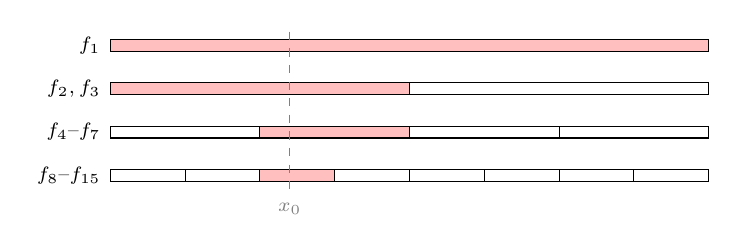
\begin{tikzpicture}[xscale=7.6, yscale=1]
  % 第 1 层 (k=0)
  \draw[fill=red!25] (0,0) rectangle (1,0.15);
  \node[left, font=\scriptsize] at (0,0.075) {$f_1$};
  % 第 2 层 (k=1)
  \draw[fill=red!25] (0,-0.55) rectangle (0.5,-0.4);
  \draw (0.5,-0.55) rectangle (1,-0.4);
  \node[left, font=\scriptsize] at (0,-0.475) {$f_2, f_3$};
  % 第 3 层 (k=2)
  \draw (0,-1.1) rectangle (0.25,-0.95);
  \draw[fill=red!25] (0.25,-1.1) rectangle (0.5,-0.95);
  \draw (0.5,-1.1) rectangle (0.75,-0.95);
  \draw (0.75,-1.1) rectangle (1,-0.95);
  \node[left, font=\scriptsize] at (0,-1.025) {$f_4$--$f_7$};
  % 第 4 层 (k=3)
  \foreach \j in {0,1,3,4,5,6,7} {
    \pgfmathsetmacro{\a}{\j/8}\pgfmathsetmacro{\b}{(\j+1)/8}
    \draw (\a,-1.65) rectangle (\b,-1.5);}
  \draw[fill=red!25] (0.25,-1.65) rectangle (0.375,-1.5);
  \node[left, font=\scriptsize] at (0,-1.575) {$f_8$--$f_{15}$};
  % 点 x_0
  \draw[dashed, gray] (0.3,0.25) -- (0.3,-1.8) node[below, font=\scriptsize] {$x_0$};
\end{tikzpicture}
\end{center}

\textbf{(红}: 每层含 $x_0$ 的小区间$)$ --- 函数值``游走''于 $0$ 与 $1$ 之间: 这就是\alert{打字机函数列}.

\end{frame}

%------------------------------------------------

\begin{frame}{打字机函数列: 处处不收敛, 却在测度意义下规矩}

\begin{itemize}
\item \textbf{处处不收敛}: $\forall\, x \in [0,1]$, 第 $k+1$ 层的 $2^k$ 个闭区间中, $x$ 至少属于\alert{1}个、至多属于\alert{2}个. 故 $\forall\, N$, 存在 $n_1, n_2 > N$ 使
\[
f_{n_1}(x) = 1, \qquad f_{n_2}(x) = 0,
\]
即 $\lim_k f_k(x)$ \alert{处处不存在}.
\end{itemize}

\pause

\begin{itemize}
\item \textbf{但坏点越来越少}: $n = 2^k + i$ 时, $E(f_n > \varepsilon)\ (0 < \varepsilon < 1)$ 含于支撑区间及其相邻区间,
\[
m\big(E(f_n > \varepsilon)\big) \leqslant \frac{2}{2^k} \longrightarrow 0
\qquad (n \to \infty,\ \text{此时}\ k \to \infty).
\]
\end{itemize}

\pause

\begin{question}
逐点意义下完全``失控''的函数列, 在``坏点集的\alert{测度}''意义下却规规矩矩 --- 这催生一个新的收敛概念.
\end{question}

\end{frame}

%------------------------------------------------

\begin{frame}{依测度收敛的定义}

\begin{Def}[依测度收敛]
设 $f, f_k$ 是可测集 $E$ 上 a.e.\ 有限的可测函数. 若
\[
\forall\, \varepsilon > 0:\quad
\lim_{k\to\infty}\ m\big(E(|f_k - f| \geqslant \varepsilon)\big) = 0,
\]
则称 $\{f_k\}$ 在 $E$ 上\alert{依测度收敛}于 $f$, 记作 $f_k \xrightarrow{m} f$ (教材记号 $f_k \Rightarrow f$).
\end{Def}

\pause

\begin{itemize}
\item \textbf{直观}: 不要求每个点收敛, 只要求\alert{坏点集} $\{|f_k - f| \geqslant \varepsilon\}$ 的\alert{测度} $\to 0$ --- 概率论中``依概率收敛''的测度论版本;
\item ``$\geqslant \varepsilon$''与``$> \varepsilon$''无区别: $E(|g| \geqslant \varepsilon) \subset E(|g| > \varepsilon/2)$;
\item 打字机列 $f_k \xrightarrow{m} 0$ 而处处不收敛 --- 依测度收敛\alert{严格更弱};
\item 定义\alert{无需} $mE < \infty$.
\end{itemize}

\end{frame}

%------------------------------------------------

\begin{frame}{a.e.\ 收敛与依测度收敛的关系}

\begin{thm}[a.e.\ $\Longrightarrow$ 依测度]
设 $mE < \infty$ 且 $f_k \xrightarrow{\text{a.e.}} f$, 则 $f_k \xrightarrow{m} f$.
\end{thm}

\startproof[bg=yellow, fg=red](证明)
由引理, $\forall\, \varepsilon > 0$:
\[
m\big(E_k(\varepsilon)\big) \leqslant m\Big(\bigcup_{l \geqslant k} E_l(\varepsilon)\Big) \longrightarrow 0
\qquad (k \to \infty).
\]
\qed

\pause

\begin{attnblock}
两个方向都不可逆:
\begin{itemize}
\item 依测度 $\not\Longrightarrow$ a.e.: 打字机函数列;
\item $mE = +\infty$ 时 a.e.\ $\not\Longrightarrow$ 依测度: $\mathbb{R}$ 上 $f_k = \chi_{[k, k+1)}$ 处处 $\to 0$, 但
$mE(|f_k| \geqslant \frac12) = 1 \not\to 0$.
\end{itemize}
依测度收敛能否至少``部分地''恢复 a.e.\ 收敛? --- \alert{Riesz 定理}.
\end{attnblock}

\end{frame}

%------------------------------------------------

\section{Riesz 定理}

%------------------------------------------------

\begin{frame}{F.~Riesz 定理}

\begin{thm}[F.~Riesz]
设 $mE < \infty$. 可测函数列 $\{f_k\}$ 依测度收敛于 $f$ 的\alert{充要条件}是: $\{f_k\}$ 的任何子列 $\{f_{k_n}\}$ 都存在进一步的子列 $\{f_{k_{n_j}}\}$ \alert{几乎处处收敛}于 $f$.
\end{thm}

\pause

\begin{itemize}
\item 依测度收敛虽不保证逐点收敛, 但\alert{子列意义下}完全恢复 a.e.\ 收敛 --- 类比: 有界数列必有收敛子列 (``紧性'');
\item ``$\Longrightarrow$'': 依测度收敛列必有 a.e.\ 收敛子列 --- 第四章积分极限定理证明中的关键工具;
\item ``$\Longleftarrow$'': 说明依测度收敛恰好是``任何子列都有 a.e.\ 收敛的进一步子列''这一性质的完全刻画.
\end{itemize}

\end{frame}

%------------------------------------------------

\begin{frame}{Riesz 定理的证明 (一): 抽子列}

\startproof[bg=yellow, fg=red]($\Longrightarrow$)
$\{f_k\}$ 的任何子列 $\{f_{k_n}\}$ 也依测度收敛于 $f$ ($m(E(|f_{k_n} - f| \geqslant \varepsilon))$ 是收敛于 $0$ 的数列的子数列), 故只需证明: \alert{依测度收敛列必有 a.e.\ 收敛子列}.

\pause

$\forall\, n \in \mathbb{N}$, 取 $\varepsilon = 2^{-n}$: 存在 $k_n$ 使
\[
m\big(E(|f_{k_n} - f| \geqslant 2^{-n})\big) < 2^{-n},
\]
逐次增大可要求 $k_1 < k_2 < \cdots$. 记
\[
E_n := E(|f_{k_n} - f| \geqslant 2^{-n}),
\qquad
E^* := \varlimsup_{n\to\infty} E_n = \bigcap_{i=1}^{\infty}\ \bigcup_{n \geqslant i} E_n .
\]

\pause

(下页: $mE^* = 0$, 且子列在 $E \setminus E^*$ 上处处收敛于 $f$.)

\qed

\end{frame}

%------------------------------------------------

\begin{frame}{Riesz 定理的证明 (二): $E \setminus E^*$ 上处处收敛}

\startproof[bg=yellow, fg=red]($\Longrightarrow$ (续))
\textbf{$E^*$ 零测}: $\forall\, i$,
\[
mE^* \leqslant m\Big(\bigcup_{n \geqslant i} E_n\Big)
\leqslant \sum_{n \geqslant i} mE_n
< \sum_{n \geqslant i} 2^{-n} = 2^{-i+1} \longrightarrow 0
\implies mE^* = 0 .
\]

\pause

\textbf{子列收敛}: 设 $x \in E \setminus E^*$, 则 $x$ 至多属于有限个 $E_n$: 存在 $i$,
\[
\forall\, n \geqslant i:\quad |f_{k_n}(x) - f(x)| < 2^{-n} \longrightarrow 0,
\]
即 $f_{k_n}(x) \to f(x)$.

\pause

故 $f_{k_n} \xrightarrow{\text{a.e.}} f$, ``$\Longrightarrow$''得证.
\qed

\end{frame}

%------------------------------------------------

\begin{frame}{Riesz 定理的证明 (三): 必要性}

\startproof[bg=yellow, fg=red]($\Longleftarrow$ 反证)
设任何子列都有 a.e.\ 收敛的进一步子列, 但 $f_k \xrightarrow{m} f$ 不成立: 存在 $\varepsilon_0 > 0$ 使
\[
a_k := m\big(E(|f_k - f| \geqslant \varepsilon_0)\big) \not\to 0 .
\]
$a_k$ 有界 ($\leqslant mE < \infty$), 故有子列 $a_{k_n} \to a \neq 0$ (若其一切收敛子列均 $\to 0$, 则 $a_k \to 0$, 矛盾).

\pause

于是对 $\{k_n\}$ 的\alert{任何}进一步子列 $\{k_{n_j}\}$: $a_{k_{n_j}} \to a > 0$, 故存在 $J$, 当 $j \geqslant J$ 时 $a_{k_{n_j}} \geqslant a/2$, 从而
\[
m\Big(\bigcup_{j \geqslant i} E(|f_{k_{n_j}} - f| \geqslant \varepsilon_0)\Big)
\geqslant \frac{a}{2} > 0 \qquad (i \geqslant J).
\]

\pause

但若 $\{f_{k_{n_j}}\}$ 有进一步的子列 a.e.\ 收敛于 $f$, 对该子列用\alert{引理}, 其尾部并的测度应 $\to 0$ --- 矛盾. 故 $\{f_{k_n}\}$ 没有任何 a.e.\ 收敛于 $f$ 的进一步子列, 与假设矛盾.
\qed

\end{frame}

%------------------------------------------------

% 依测度极限的唯一性 (属 Riesz 定理一节)

\begin{frame}{依测度极限的唯一性}

\begin{thm}[唯一性]
若 $\{f_k\}$ 在 $E$ 上同时依测度收敛于 $f$ 与 $g$, 则 $f \sim g$ (即 $f = g$ a.e.).
\end{thm}

\startproof[bg=yellow, fg=red](证明)
逐点有 $|f - g| \leqslant |f - f_k| + |g - f_k|$, 故 $\forall\, \varepsilon > 0$:
\[
E(|f - g| \geqslant \varepsilon)
\subset E(|f - f_k| \geqslant \tfrac{\varepsilon}{2})
\cup E(|g - f_k| \geqslant \tfrac{\varepsilon}{2}).
\]

\pause

取测度并令 $k \to \infty$:
\[
m\big(E(|f - g| \geqslant \varepsilon)\big) = 0, \qquad \forall\, \varepsilon > 0.
\]

\pause

由 $\varepsilon$ 的任意性 ($E(|f-g| > 0) = \bigcup_{n} E(|f - g| \geqslant \frac1n)$):
$mE(|f - g| > 0) = 0$, 即 $f \sim g$.
\qed

\pause

\textbf{解读}: 依测度收敛一般没有逐点极限, 但其``极限''在 \alert{a.e.\ 等价类}意义下唯一 (\S 3.1 的 $f \sim g$ 语言) --- 可以放心谈论``依测度极限''.

\end{frame}

%------------------------------------------------

\section[完备性]{依测度基本列与完备性}

%------------------------------------------------

\begin{frame}{依测度基本列}

\begin{Def}[依测度基本列]
设 $\{f_k\}$ 是可测集 $E$ 上 a.e.\ 有限的可测函数列. 若
\[
\forall\, \varepsilon > 0:\quad
\lim_{i,\, j \to \infty}\ m\big(E(|f_i - f_j| \geqslant \varepsilon)\big) = 0,
\]
则称 $\{f_k\}$ 为 $E$ 上的\alert{依测度基本列} (依测度 Cauchy 列).
\end{Def}

\pause

\begin{itemize}
\item 与度量空间的 Cauchy 列完全类比: 依测度收敛 $\Longrightarrow$ 依测度基本列 (三角不等式);
\item \alert{逆命题} (完备性) 是本节的主题 --- 类比 $\mathbb{Q}$ 中 $\sqrt2$: 没有完备性的空间里, 基本列可能没有极限;
\item 甚至可定义 Fr\'echet 度量 $d(f, g) = \displaystyle\inf_{\varepsilon > 0} \big(\varepsilon + mE(|f - g| > \varepsilon)\big)$, 依测度收敛即 $d(f_k, f) \to 0$ (选学).
\end{itemize}

\end{frame}

%------------------------------------------------

\begin{frame}{完备性定理}

\begin{thm}[完备性]
设 $mE < \infty$, $\{f_k\}$ 是 $E$ 上的依测度基本列. 则存在 $E$ 上 a.e.\ 有限的可测函数 $f$, 使 $f_k \xrightarrow{m} f$.
\end{thm}

\pause

\startproof[bg=yellow, fg=red](证明 (一): 抽子列)
由基本列定义, 可选 $k_1 < k_2 < \cdots$ 使
\[
m\big(E(|f_{k_{n+1}} - f_{k_n}| \geqslant 2^{-n})\big) < 2^{-n},
\qquad \forall\, n \in \mathbb{N}
\]
(依次取 $\varepsilon = 2^{-n}$ 对应的 $N$, 并让 $k_{n+1}$ 足够大).

\pause

记 $E_n := E(|f_{k_{n+1}} - f_{k_n}| \geqslant 2^{-n})$, $E^* = \varlimsup_{n} E_n$. 与 Riesz 定理同理:
\[
mE^* \leqslant m\Big(\bigcup_{n \geqslant i} E_n\Big)
\leqslant \sum_{n \geqslant i} 2^{-n} \longrightarrow 0
\implies mE^* = 0 .
\]
(下页: 定义极限函数 $f$.)

\qed

\end{frame}

%------------------------------------------------

\begin{frame}{完备性定理的证明 (二): 定义 $f$ 并验证}

\startproof[bg=yellow, fg=red](证明 (二))
$x \in E \setminus E^*$: 存在 $i$, $\forall\, n \geqslant i$: $|f_{k_{n+1}}(x) - f_{k_n}(x)| < 2^{-n}$, 于是当 $m > n \geqslant i$:
\[
|f_{k_m}(x) - f_{k_n}(x)|
\leqslant \sum_{l=n}^{m-1} 2^{-l} < 2^{-n+1} \longrightarrow 0,
\]
即 $\{f_{k_n}(x)\}$ 是 $\mathbb{R}$ 中的基本列, 必收敛. 定义
\[
f(x) := \begin{cases}
\lim\limits_{n\to\infty} f_{k_n}(x), & x \in E \setminus E^*,\\[0.4em]
0, & x \in E^* .
\end{cases}
\]
$f$ 可测 (处处收敛的可测函数列的极限, \S 3.1) 且 a.e.\ 有限.

\pause

\textbf{验证 $f_k \xrightarrow{m} f$}: 对 $i$ 与所选子列,
\[
E(|f_i - f| \geqslant \varepsilon)
\subset E(|f_i - f_{k_i}| \geqslant \tfrac{\varepsilon}{2})
\cup E(|f_{k_i} - f| \geqslant \tfrac{\varepsilon}{2}).
\]
前者: $i, k_i \to \infty$, 基本列性质 $\Rightarrow$ 测度 $\to 0$; 后者: $f_{k_i} \xrightarrow{\text{a.e.}} f$ 且 $mE < \infty$ $\Rightarrow$ 依测度收敛 $\Rightarrow$ 测度 $\to 0$. 故 $f_k \xrightarrow{m} f$.
\qed

\pause

\textbf{手稿注记}: $f$ 也可写成级数 $f = f_{k_1} + \sum_{n \geqslant 1} (f_{k_{n+1}} - f_{k_n})$ --- 部分和是可测函数, 由此亦可看出 $f$ 可测.

\end{frame}

%------------------------------------------------

\section[运算性质]{依测度极限的运算性质}

%------------------------------------------------

\begin{frame}{依测度极限的运算性质}

\begin{thm}[运算性质]
设 $f_k \xrightarrow{m} f$, $g_k \xrightarrow{m} g$ (均在 $E$ 上). 则
\begin{itemize}
\item[(1)] $a f_k + b g_k \xrightarrow{m} a f + b g$ \ ($a, b \in \mathbb{R}$);
\item[(2)] $|f_k| \xrightarrow{m} |f|$;
\item[(3)] $\max(f_k, g_k) \xrightarrow{m} \max(f, g)$, \quad $\min(f_k, g_k) \xrightarrow{m} \min(f, g)$.
\end{itemize}
\end{thm}

\pause

\startproof[bg=yellow, fg=red](证明 (1)(2))
(1) 若 $|af_k + bg_k - (af + bg)| \geqslant \varepsilon$, 则 $|a|\,|f_k - f| \geqslant \frac{\varepsilon}{2}$ 或 $|b|\,|g_k - g| \geqslant \frac{\varepsilon}{2}$, 故
\[
E\big(|af_k + bg_k - (af+bg)| \geqslant \varepsilon\big)
\subset E\big(|f_k - f| \geqslant \tfrac{\varepsilon}{2|a|}\big)
\cup E\big(|g_k - g| \geqslant \tfrac{\varepsilon}{2|b|}\big),
\]
右端测度 $\to 0$ ($a = 0$ 或 $b = 0$ 时平凡).

(2) $\big||f| - |f_k|\big| \leqslant |f - f_k|$, 故
$E\big(\big||f| - |f_k|\big| \geqslant \varepsilon\big) \subset E(|f - f_k| \geqslant \varepsilon)$.
\qed

\end{frame}

%------------------------------------------------

\begin{frame}{运算性质的证明 (3): 化为已证情形}

\startproof[bg=yellow, fg=red](证明 (3))
逐点成立的初等恒等式:
\[
\max(f, g) = \frac{f + g + |f - g|}{2},
\qquad
\min(f, g) = \frac{f + g - |f - g|}{2}.
\]

\pause

于是
\[
\max(f_k, g_k) - \max(f, g)
= \frac{(f_k - f) + (g_k - g) + \big(|f_k - g_k| - |f - g|\big)}{2}.
\]
由 (1): $(f_k - f) + (g_k - g) \xrightarrow{m} 0$; 由 (1)(2): $|f_k - g_k| \xrightarrow{m} |f - g|$. 再用 (1) 合并, 得
$\max(f_k, g_k) \xrightarrow{m} \max(f, g)$; $\min$ 同理 (改变末项符号).
\qed

\pause

\begin{remark}
这与 \S 3.1 中``$\max/\min$ 可测''的证明用的是\alert{同一恒等式} --- 同一手法, 两个场合. 结合 (1)(2)(3): 依测度极限对\alert{线性组合、绝对值、格运算}全部封闭.
\end{remark}

\end{frame}

%------------------------------------------------

\section[小结]{小结与展望}

%------------------------------------------------

\begin{frame}{收敛概念的层次 ($mE < \infty$)}

\begin{center}
\begin{tikzpicture}[yscale=1.15]
  \node (u)  at (0,0)     {\footnotesize 一致收敛};
  \node (au) at (3.1,0)   {\footnotesize 近一致收敛};
  \node (ae) at (6.4,0)   {\footnotesize a.e.\ 收敛};
  \node (m)  at (9.6,0)   {\footnotesize 依测度收敛};
  \draw[->] (u)  -- (au);
  \draw[->] (au) -- (ae) node[midway, above, font=\tiny] {注记(二)};
  \draw[->] (ae) -- (m)  node[midway, above, font=\tiny] {$mE<\infty$};
  \draw[->] (ae) to[bend left=30] node[below, font=\tiny] {Egorov ($mE<\infty$)} (au);
  \draw[->, dashed] (m) to[bend left=45] node[above, font=\tiny] {Riesz: 可抽 a.e.\ 收敛子列} (ae);
\end{tikzpicture}
\end{center}

\pause

\begin{itemize}
\item 一致 $\Longrightarrow$ 近一致 (取 $E_\delta = E$); 反向不行: $f_k(x) = x^k$ 于 $[0,1]$;
\item 依测度 $\not\Longrightarrow$ a.e.: 打字机函数列 --- 新概念\alert{严格更弱};
\item $mE = +\infty$ 时链条断裂: $\chi_{[k, k+1)}$ 于 $\mathbb{R}$ 处处 $\to 0$, 但既不近一致收敛, 也不依测度收敛;
\item 唯一性: 依测度极限在 $f \sim g$ 意义下唯一; 完备性: 依测度基本列必有依测度极限.
\end{itemize}

\end{frame}

%------------------------------------------------

\begin{frame}{小结}

\begin{itemize}
\item \textbf{集列语言}: $\varlimsup A_n$ = ``属于无穷多次'', $\varliminf A_n$ = ``最终恒属于''; 函数列不收敛点集用坏集合列的上极限控制;
\pause
\item \textbf{引理} (a.e.\ 收敛的测度刻画): $m(\bigcup_{k \geqslant n} E_k(\varepsilon)) \to 0$ --- 证明靠\alert{渐缩集列}的连续性 ($mE_1 < \infty$!), 它是 Egorov 与 Riesz ($\Longleftarrow$) 的共同引擎;
\pause
\item \textbf{Egorov 定理}: $mE < \infty$ 时 a.e.\ 收敛 $\iff$ 近一致收敛; 但近一致 $\neq$ 一致 ($x^k$); \alert{各 $f_k$ 连续时 $f\big|_{E_\delta}$ 连续} ($\varepsilon/3$) --- Luzin 定理雏形;
\pause
\item \textbf{依测度收敛}: 打字机例; a.e.\ $\Longrightarrow$ 依测度 ($mE < \infty$); Riesz 子列定理; 极限 a.e.\ 唯一; 依测度基本列必有极限 (\alert{完备性}); 对线性组合、$|\cdot|$、$\max/\min$ 封闭.
\end{itemize}

\end{frame}

%------------------------------------------------

\begin{frame}{展望}

\begin{itemize}
\item \textbf{\S 3.3 可测函数的构造}: Luzin 定理 --- 可测函数``挖掉小测度集后连续'', 即\alert{可测 $\approx$ 连续}; 证明核心正是 Egorov 定理 + 本节选讲的``连续性继承'';
\pause
\item \textbf{\S 4 勒贝格积分}: 极限与积分换序的定理 (Lebesgue 控制收敛定理等) 中, ``依测度收敛 + Riesz 抽子列''是标准起手式; 依测度收敛的完备性保证了各种收敛概念的衔接;
\pause
\item \textbf{概率论}: 依测度收敛 = 依概率收敛; Egorov / Riesz 在概率语言下即``几乎必然收敛 $\to$ 依概率收敛''与``依概率收敛必有几乎必然收敛的子列''.
\end{itemize}

\end{frame}

%------------------------------------------------

\ifIncludeExercise
\begin{frame}{作业}

\begin{block}{教材第三章 \S 3.2 习题}
\begin{itemize}
\item \textbf{13.} 试给出关于可测函数列当极限函数为无穷大情形的相应 Egorov 定理的陈述并加以证明.
\item \textbf{14.} 设 $x \in [0, 1)$, 其二进表示为 $x = \sum_{i=1}^{\infty} \frac{x_i}{2^i}$ ($x_i \in \{0, 1\}$, 约定用有尽表示). 定义函数 $\varphi(x) = \sum_{i=1}^{\infty} \frac{2x_i}{3^i}$, 再取 $[0, 1)$ 的一不可测子集 $E$, 并在 $\mathbb{R}$ 上定义函数 $\psi(x) = 1$ (当 $x \in \varphi(E)$), $\psi(x) = 0$ (其余情形). 试证 $\varphi, \psi$ 均可测, 但 $\psi \circ \varphi$ 不可测.
\item \textbf{17.} 设函数列 $\{f_n\}$ 在 $E$ 上依测度收敛于 $f$, 且在 $E$ 上几乎处处有 $f_n \leqslant g$ ($n \in \mathbb{N}$). 试证在 $E$ 上几乎处处有 $f \leqslant g$.
\item \textbf{21.} 试构造 $[0, 1]$ 上的连续函数列 $\{f_n\}$, 使满足 (i) $\{f_n\}$ 在 $[0,1]$ 上几乎处处收敛于 $0$, 但 (ii) $\{f_n\}$ 在任何子区间上不一致收敛于 $0$.
\item \textbf{26.} 设函数列 $\{f_n\}$ 在 $\mathbb{R}$ 上几乎处处收敛于有限函数 $f$. 试证存在可测集列 $\{E_k\}$, 使在每个 $E_k$ 上 $\{f_n\}$ 一致收敛于 $f$ ($n \to \infty$), 而 $\mathscr{C}\big(\bigcup_{k=1}^{\infty} E_k\big)$ 为零测集.
\end{itemize}
\end{block}

\end{frame}
\fi

%------------------------------------------------

\end{document}
